\documentclass{article}
\linespread{1.25}

\usepackage{pgfplots}
\pgfplotsset{compat=1.18}

\usepackage[top = 2cm, right=2cm, left=2cm]{geometry}
\usepackage{graphicx}
\usepackage[section]{placeins}
\usepackage[hidelinks, urlcolor=blue]{hyperref}
\usepackage{float} % for image position in exatly where you want
\usepackage[perpage, stable]{footmisc}
\usepackage{amsmath}
\usepackage{titling}

\usepackage{xepersian}
\settextfont{B Nazanin}
\setlatinmonofont{CMU Serif}
%\setlatinmonofont{Times New Roman}
\setlatintextfont{Times New Roman}

% Set Latin Modern font for the bullets in itemizea
\newfontfamily\latinbullet{Latin Modern Roman}





% Commands
\newcommand{\column}[1]{\lr{\textit{#1}}}
\renewcommand{\labelitemi}{{\latinbullet\textbullet}} % Use the bullet from Latin Modern font

% Custom title page setup
\makeatletter
\def\maketitle{
	\begin{titlepage}
		\begin{center}
			\vspace*{2cm}
			
			{\Large\bfseries درس یادگیری ماشین\par}
			\vspace{2cm}
			
			{\Huge\bfseries پاسخ تکلیف
				\lr{Linear Regression}\par}
			\vspace{3cm}
			
			{\large\bfseries استاد درس:\par}
			{\large دکتر افتخاری\par}
			\vspace{1.5cm}
			
			{\large\bfseries نگارش:\par}
			{\large امیرحسین ابوالحسنی\par}
			{\large شماره دانشجویی: 400405003\par}
			\vspace{2cm}
			
			\vfill  % pushes the date to bottom
			
			{\large\bfseries پاییز \lr{1403}}
			
		\end{center}
	\end{titlepage}
	\setcounter{page}{1}
}
\makeatother


\begin{document}
	\maketitle	
	\section*{سوال 1}
	\subsection{نمودار پراکندگی}
	\begin{center}
		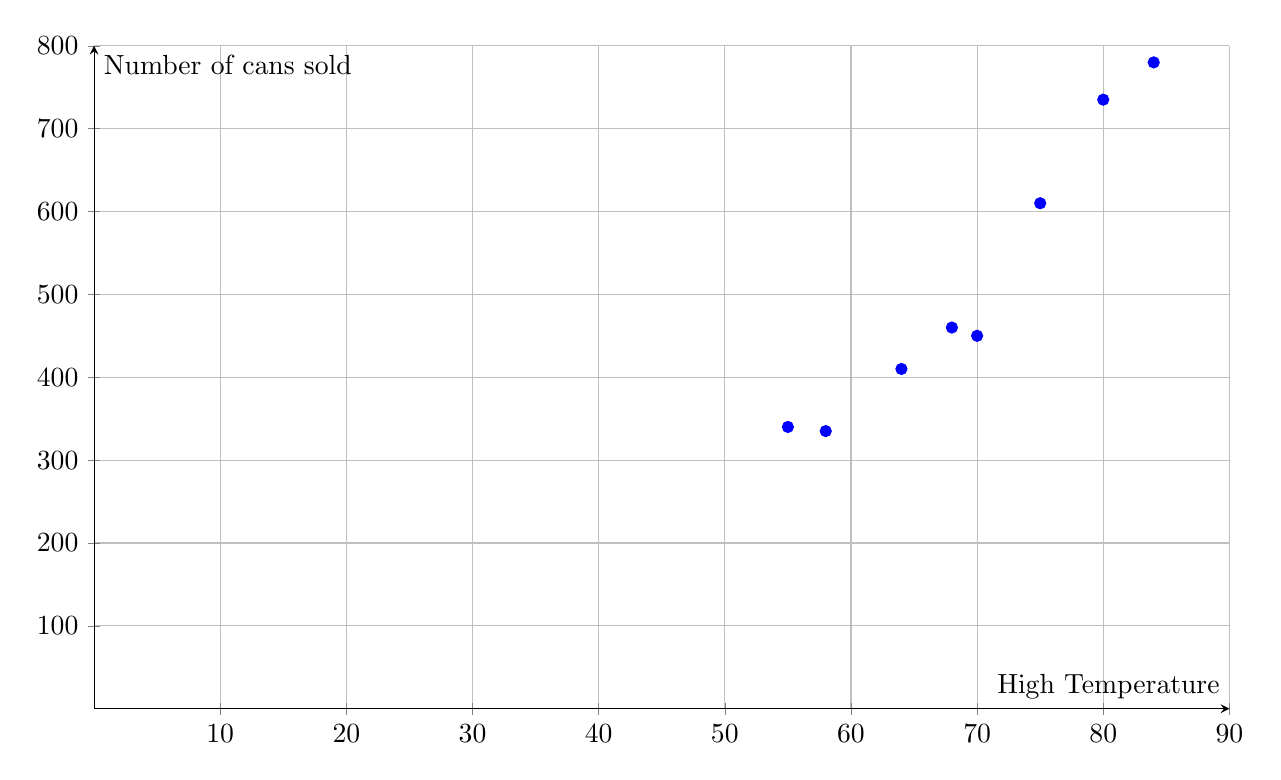
\begin{tikzpicture}
			\begin{axis}[
				xlabel={\lr{High Temperature}},
				ylabel={\lr{Number of cans sold}},
				grid=major,
				width=16cm,
				height=10cm,
				xmin=0, xmax=90,  % Set the x-axis range
				ymin=0, ymax=800,  % Set the y-axis range
				axis lines=middle, % Place the axes at the origin
				]
				\addplot[
				only marks,
				mark=*,
				color=blue,
				] coordinates {
					(55, 340)
					(58, 335)
					(64, 410)
					(68, 460)
					(70, 450)
					(75, 610)
					(80, 735)
					(84, 780)
				};
			\end{axis}
		\end{tikzpicture}
	\end{center}
	\subsection{معادله و رسم یک رگرسیون خطی برای داده ها}
	برای به دست آوردن پارمتر‌های رگرسیون داریم:
	\begin{flalign*}
		\theta  & = (X^TX)^{-1}X^T\vec{y}\\
				& = (\begin{pmatrix}
					1&1&1&1&1&1&1&1 \\
					55& 58& 64& 68& 70& 75& 80 & 84
				\end{pmatrix}
				\begin{pmatrix}
					1 & 55\\
				1 & 58\\
				1 & 64\\
				1 & 68\\
				1 & 70\\
				1 & 75\\
				1 & 80\\
				1 & 84
				\end{pmatrix})^{-1}
				\begin{pmatrix}
					1&1&1&1&1&1&1&1 \\
					55& 58& 64& 68& 70& 75& 80 & 84
				\end{pmatrix}
				\begin{pmatrix}
					340\\
					335\\
					410\\
					460\\
					450\\
					610\\
					735\\
					780
				\end{pmatrix}\\
				& = \begin{pmatrix}
					8 & 554\\
					554 & 39090
				\end{pmatrix}^{-1}
				\begin{pmatrix}
					4120 \\
					297220
				\end{pmatrix}\\
				& = \begin{pmatrix}
					6.73501034 & -0.0954514128\\
					-0.0954514128 &‌0.00137835975
				\end{pmatrix}
				\begin{pmatrix}
					4120 \\
					297220
				\end{pmatrix}\\
				& = \begin{pmatrix}
					-621.82632667\\
					16.41626465
				\end{pmatrix}
	\end{flalign*}
	پس خطی داریم به معادله:
	\[ -621.82632667 + 16.41626465 ~ x = y \]
	و به شکل:
	\begin{center}
		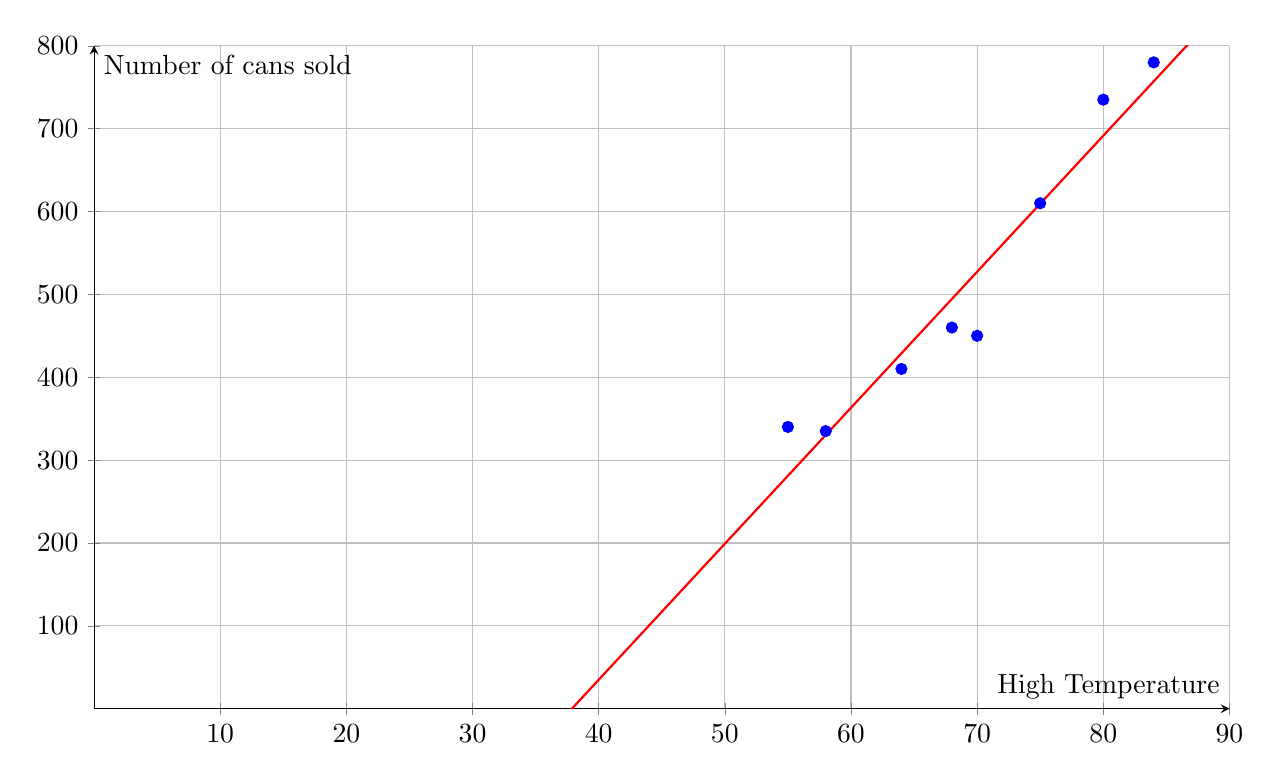
\begin{tikzpicture}
			\begin{axis}[
				xlabel={\lr{High Temperature}},
				ylabel={\lr{Number of cans sold}},
				grid=major,
				width=16cm,
				height=10cm,
				xmin=0, xmax=90,  % Set the x-axis range
				ymin=0, ymax=800,  % Set the y-axis range
				axis lines=middle, % Place the axes at the origin
				]
				\addplot[
				only marks,
				mark=*,
				color=blue,
				] coordinates {
					(55, 340)
					(58, 335)
					(64, 410)
					(68, 460)
					(70, 450)
					(75, 610)
					(80, 735)
					(84, 780)
				};
				
				\addplot[
				domain=0:100, % Range for x-axis
				samples=2,  % Number of points for smoothness
				thick,
				color=red,
				] {-621.82632667 + 16.41626465*x}; % Replace with your line equation
			\end{axis}
		\end{tikzpicture}
	\end{center}
	\subsection{}
	\section*{سوال 2}
	\section*{سوال 3}
	\section*{سوال 4}
	
	
\end{document}